\chapter{Attacks on \KECCAK{}}

In this chapter we study various attacks on \KECCAK{}.The following are the basic types of attacks which are applicable to a cryptographic hash function:

\begin{enumerate}
	\item \textbf{Preimage Attacks}
	\item \textbf{Collision Attacks}
	\item \textbf{Second-Preimage Attacks}
\end{enumerate}
Now, we will discuss these types of attack in detail.

\section{Preimage Attacks on Round Reduced Keccak}

In a Preimage attack, the attacker is able to derive message from the digest of the hash function. For a n-bit hash value in general it takes $O(2^{n})$ computations to compute the message but this a brute-force attack. These kind of attacks are avoided by designers of hash function by setting the size of digest accordingly. An attack with complexity greater than or equal to $O(2^{80})$ is considered computationally hard to achieve. The makers of \KECCAK{} have released various variants of the hash function \SHA-3 with different sizes of output hash. The 4 \SHA-3 functions are \SHA3-224, \SHA3-256, \SHA3-384 and \SHA3-512, with these lengths of hash value it's a hard to compute a preimage. Cryptographers across the globe are working on breaking the reduced round versions of \KECCAK{} by providing practical preimage attacks for these four \SHA-3 hash functions. Till date there are practical preimage attacks only for $3$ rounds of \KECCAK-$224$, $2$ rounds of \KECCAK-$256$ and $1$ round of \KECCAK-$384$, \KECCAK-$512$. There are still no practical preimage attacks for $2$ rounds of \KECCAK-$384$, \KECCAK-$512$. These preimage attacks provided by various cryptographers involve cryptanalysis of the underlying transformations per round and try to control there behaviour in some way and get the values of message variables.

There are some improved preimage attacks for $2$ rounds of \KECCAK-$384$, \KECCAK-$512$ proposed by Guo \etal in ~\cite{guo2016linear} which have complexities better than brute-force attacks but are still not practical. Similarly there are many theoretical attacks on four \SHA-3 functions for different number of rounds which are better than brute-force. Improving and achieving practical preimage attacks for reduced round variants of \KECCAK{} is an active area of research and in this thesis, we address the same.

In \cite{guo2016linear}, Guo \etal describe there techniques for preimage attacks where they use linear structures to linearize variables up to 3 rounds. The Linear structures are the states of \KECCAK{} state which have a certain number of free linear variables, these free variables provide us with degrees of freedom which help in improving over brute-force attacks. These free variables form the linear structure. So, the more number of free variables the better complexity of attack we can achieve provided the system of equations remains linear.

In this type of attack, we set message variables in the rate part in such a way that the state remains a linear structure for the number of required rounds. Here, we go forwards with the message variables for (number of rounds - 1) + half round, considering the state is linear structure and rest of round we go backwards from the hash, and then build a system of linear equations and solve it to get the values of message variables. So, after a message is found from the hash we get the preimage successfully. This is a meet in the middle approach of attacking the system.

\section{Preimage Attacks on 2-round \KECCAK}

In this section we will discuss some of the existing Preimage attacks on 2 rounds of round-reduced \KECCAK{}. The figure~\ref{fig:linkeccakstate} used for denoting \KECCAK{} state, the numbers $x,y$ in each cell denotes the position of these lanes in the state.

\begin{figure}
    \centering
    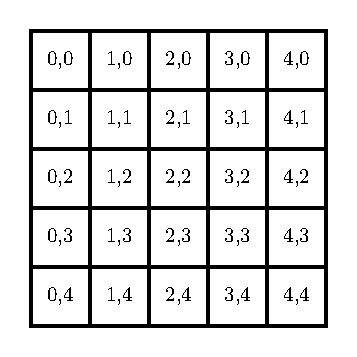
\includegraphics{keccakState.pdf}
    \caption{\KECCAK{} State with lane position specified}
    \label{fig:linkeccakstate}
\end{figure}


\subsection{Preimage Attacks on 2-round \KECCAK-$512$}
		This attack is for 2 rounds of \KECCAK-$512$, it uses meet in the middle approach. The 1st-round is kept linear by linear structure and the last round i.e. the second round is inverted from the given hash value. From the given hash, they invert $\iota$ as its the simple addition of round constant for the particular round, followed by inverting only row-$0$ by $\chi$ operation. This attack is for \KECCAK-$512$, so the hash length is $512$ i.e. $8$ lanes. Since $\chi$ operation is like a Sbox for a $row$, they invert the first row using the Observation~\ref{ob1}. So till now we have the values of the first row of the state just before last round steps $\iota \circ \chi$. Now, they focus on proceeding one round forward, so they start with empty state where they fix lanes $(0,0), (0,1), (2,0) $ and $(2,1)$ as variables, rest of the part of the $rate$ is assigned random value and the $capacity$ part remains $0$ as shown in figure~\ref{fig:2rkeccak512} where yellow colored lanes are ones which are taken as variables i.e. $(0,0), (0,1)$ in column $0$ and $(2,0), (2,1)$ in column $2$. Also, the structure of the states in this figure is the same as~\ref{fig:linkeccakstate}. White lanes are set as any random value and gray lanes are the zero lanes in the $capacity$ part in figure~\ref{fig:2rkeccak512}.
		\begin{figure}
            \centering
            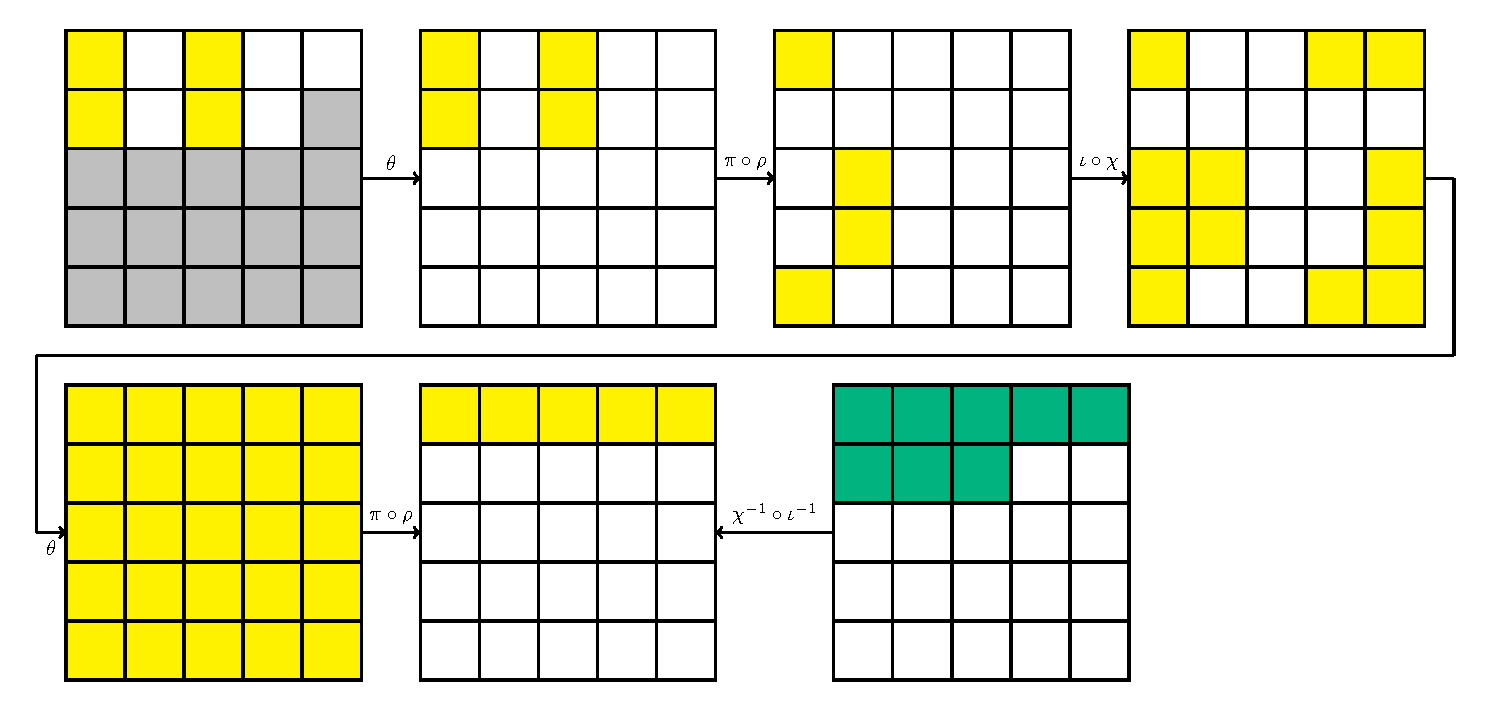
\includegraphics[scale=0.6]{2Rkeccak512.pdf}
            \caption{Preimage Attack on 2-round \KECCAK-$512$}
            \label{fig:2rkeccak512}
        \end{figure}
	    To avoid the spreading of linear variables by $\theta$ they impose the following conditions : 
		\[
			A[0, 1] = A[0, 0] \oplus \alpha_{0}
		\]
		\[
			A[2, 1] = A[2, 0] \oplus \alpha_{2}
		\]
		with $\alpha_0$ and $\alpha_2$ as random constants.
		Then they proceed forward with 1-round and the state remains linear, even after 2nd round's $\pi \circ \rho \circ \theta$ the state remains linear, since these are linear operations. They then build a system of linear equations from the equations of first row of the obtained state and the values of these lanes recovered after $\chi^{-1} \circ \iota^{-1}$. After this they move on to solving the system of linear equations and verifying the obtained hash is same as the hash taken for the preimage attack, if correct a preimage is found.
		
		In the above method, initially there were 4 variables lanes and after imposing 2 conditions for $\theta$, we are left with 2 free variables each of 64-bit namely $A[0,0]$ and $A[2, 0]$. So we observe a complexity gain over brute-force by size of the free variables.
		
		Hence the complexity of the attack comes out to be $2^{512 - 64 - 64} = 2^{512 - 128} = 2^{384}$.

		For an attack to be possible, the degrees of freedom should be greater than $512$. We have 5 random white lanes, 2 variable lanes and 2 random constants, and all of these are of size $w$ which is $64$ in our discussion. So total degree of freedom comes out to be $= 9 * 64 = 576$ which is greater than $512$ which implies that a solution is possible.

\subsection{Preimage Attacks on 2-round \KECCAK-$384$}
	This attack is very similar to the above attack for \KECCAK-$512$. We start with 6 variable lanes such that :
	$A[0, 2] = A[0, 0] \oplus A[0, 1] \oplus \alpha_0$ and $A[2, 2] = A[2, 0] \oplus A[2, 1] \oplus \alpha_2$, so that $\theta$ doesn't spread and proceed for the $1.5$ rounds forward and proceed backwards from the hash by applying $\chi^{-1} \circ \iota^{-1}$. Then build a system of linear equations of 256-bit equations and solve for message variables. Then check the hash obtained is correct. So we observe a complexity gain over brute-force by size of the free variables hence the complexity of the attack comes out to be $2^{384 - 4*64} = 2^{384 - 256} = 2^{128}$. To meet the padding requirements in worst case the complexity will be $2^{129}$.

\subsection{Preimage Attacks on 2-round \KECCAK-$256$}\label{section2RKeccak256}
    \begin{figure}
        \centering
        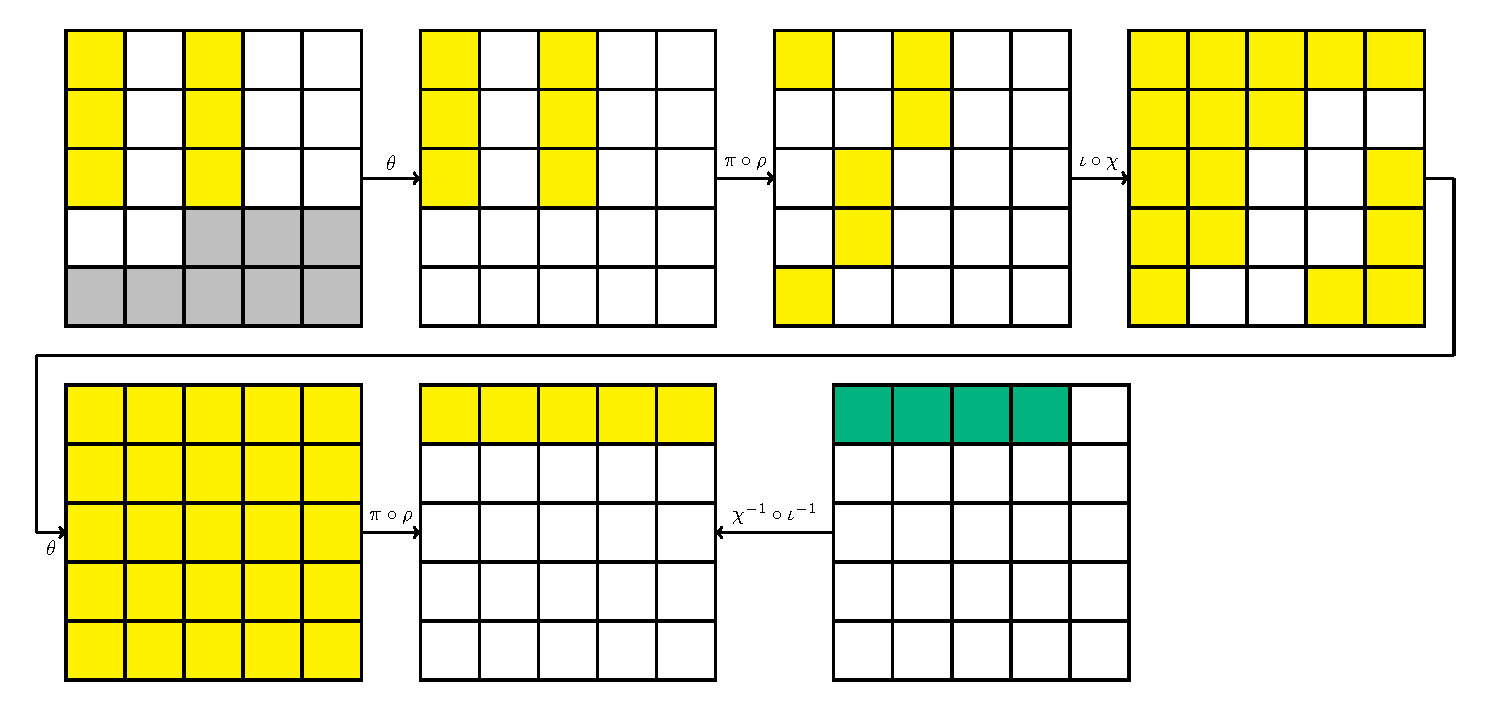
\includegraphics[scale=0.6]{2Rkeccak256.pdf}
        \caption{Preimage Attack on 2-round \KECCAK-$256$}
        \label{fig:2rkeccak256}
    \end{figure}
	The attack for 2 round \KECCAK-$256$ is very similar to the attack for \KECCAK-$384$.
	The message here is in lanes $(0, 0), (0, 1), (0, 2), (2, 0), (2, 1), (2, 2)$, rest all lanes can take any constant value as shown in figure~\ref{fig:2rkeccak256}. We keep the sum of variables in columns $0$ and $2$ constant by choosing the sum of variables in the column to be $\alpha_0$ and $\alpha_2$ respectively, where $\alpha_0, \alpha_2$ are random constants. Due to this condition the parity of column $0, 2$ is constant and $\theta$ step would affect the full state only by a constant.
	
	For \KECCAK-$256$, length of digest is $d = 256 \rightarrow 4$ lanes and capacity $c = 512 \rightarrow 8$ lanes. We can get $4$ linear equations on the input bits of $\chi$ given $4$ output bits out of the $5$-bits Observation~\ref{ob3}. Therefore, we need 4 variables in our state to build a linear system of 256-bit equation.	We have $h_0, h_1, h_2, h_3$  hash lanes in the output. By using property of $\chi$, we can get 4 linear equations on the input to the $\chi$ when 4 output bits are given. The above is true for each lane in row 0. i.e. we can get $4*64$ linear equations on the input to the $\chi$. So in one slice, we need 4 variables to map them to 4 output bits given. (according to $\chi$) 
	
	So we build initial state such that we have $4*64$ free variables. So take the same structure as for 2R, \KECCAK-$384$
	Take $A[0, 2] = A[0, 0] \oplus A[0, 1] \oplus \alpha_0$
	and $A[2, 2] = A[2, 0] \oplus A[2, 1] \oplus \alpha_2$
	The state remains linear after 1 round and 1 $L$ i.e. $\pi \circ \rho \circ \theta$, initially there were 6 variable lanes and after imposing 2 conditions for $\theta$, we are left with $4$ free variables each of 64-bit namely $A[0,0], A[0,1], A[2, 0], A[2,1]$ i.e. the linear structure.
	So, we observe a complexity gain over brute-force by size of linear structure, hence the time complexity of attack $ = 2^{256 - 256} = 2^{0} = 1$
	
	By solving the system of linear equations we get a solution in constant time. Though earlier in 2011 a practical attack was proposed in ~\cite{naya2011practical} but of complexity $2^{33}$ and by the method of linear-structures Guo \etal ~\cite{guo2016linear} were able to give preimage in constant time.

\section{Preimage Attacks on 3-round \KECCAK}

In this section we will discuss some of the existing Preimage attacks on 3 rounds of round-reduced \KECCAK{}.

\subsection{Preimage Attacks on 3-round \KECCAK-$384$, \KECCAK-$512$}

		The 3 rounds can be summarized as :
    
    $ M \xrightarrow[\text{1.5 rounds}]{ \pi \circ \rho \circ \theta \circ R} A \xrightarrow[]{ \iota \circ \chi } B \xrightarrow[]{ \theta } C \xrightarrow[]{ \pi \circ \rho } | \xleftarrow[]{ \chi^{-1} \circ \iota^{-1} } h  $

		For 3-round \KECCAK-$512$, they extend the attack mentioned for 2-round \KECCAK-$512$. They start with 4 variable lanes but after first $\theta$ only 2 variable lanes are left so that the effect of $\theta$ is constant. So, we have $128$ variable bits. Then $\pi \circ \rho$ just permutate the variable lanes and after $\chi$ the no. of linear terms increases. So after first round almost all columns have atleast one variable lane (except the 3rd column as shown in figure~\ref{fig:2rkeccak512} ). The no. of linear terms are increased such that after $\theta$ of second round the full state becomes linear. So, After $\theta$ of second round the full state becomes linear, and the $\pi \circ \rho$ further don't introduce any non-linear term, they only change the positions of lanes and rotate them, so the state is still linear.  These are first 1.5 rounds of \KECCAK{} where 0.5 round includes only the first three step mappings i.e $\theta, \rho, \pi$. Hence the state after 1.5 rounds i.e. $A$ remains linear.
		
		Following this is the $\chi$ of the second round, since the input to $\chi$ is linear terms and as we know $\chi$ is a non-linear operation so the output state after $\chi$ is a non-linear i.e. quadratic state. Dealing with non-linear terms is not easy, so the idea is to linearize the quadratic terms and try to reduce the complexity compared to brute-force attack.

		So, The bits input to step $\chi$ of the second round are all linear. We can directly inverse first 320 bits through $\chi^{-1}$ from a given hash value (8 lanes). Of the inverted state, each bit is a sum of 11 bits of the output of the second round though they will be permuted by $\rho, \pi$.

    As in section 6.3 ~\cite{guo2016linear} per equation (14) the equation of $C[x][y][z]$
    Expanding it :

    \[
        C[x][y][z] = B[x][y][z] \oplus \oplus_{y' = 0}^{4} B[x-1][y'][z] \oplus \oplus_{y' = 0}^{4} B[x+1][y'][z-1]
    \]
    
		Open all the expressions and separate two terms $B[x][y][z]$ and $B[x-1][y][z]$ and rest 9 terms remain as it is.
    So, 
		\[ B[x][y][z] \oplus B[x-1][y][z] = (a \oplus c + b) \oplus d
    \]
    Where,
		 \[
        a = A[x][y][z], b = A[x + 1][y][z], c = A[x + 2][y][z], d = A[x - 1][y][z]
    \]
    So guessing $b$ and other 9 terms would make $C[x][y][z]$ linear. Hence, We linearize $C[x][y][z]$ by guessing 10 bits input to step $\chi$. That is, we obtain 1 + 10 linear equations, by these linear equations we can match the hash value bit corresponding to $C[x][y][z]$. So 11 linear equations for 1 bit of hash value. For $\KECCAK$-$512$ we have only 128 variable bits, so we can match $128/11 = 11$ bits of the hash value.
    
    Time complexity of preimage attack $= 2^{512 - 11} = 2^{501}$.

    \textbf{Note:} There is an improvement for the above attack mentioned in 6.3 by which attack complexity is $= 2^{482}$.

    Similarly for $\KECCAK$-$384$, we have 4 variable lanes i.e. $A[0,0], A[0,1], A[2,0], A[2,1]$ left but we need to set last bit of $A[2,2]$ to $1$ to satisfy padding rules. Hence we are left with $4*64 - 1 = 255$ variable bits.
	
	No. of matched hash bits $ = 255/11 = 23 $. Time complexity of preimage attack $= 2^{384 - 23} = 2^{361}$.

\subsection{Improvements for Preimage Attacks on 3-round \KECCAK-$384$, \KECCAK-$512$}

    The idea for improvements of these attacks is an extension for the method described in previous section. As the variable bit $C[x][y][z]$ is linearized by guessing 10 bits. They assumed there that the guessing was independent, which can be dependent too if chosen properly. So the idea is to guess for those bits which would help in reducing the number of guesses for some other bit(s). So it will be possible to reduce the complexity further by choosing linearly dependent bits, so that there can be more matched bits of the hash value.

		We start with following two equations, $B$ represents the state after $\chi$ as shown in the flow diagram for 3 rounds.
		\[
			B[x][y][z] = A[x][y][z] \oplus (A[x+1][y][z] \oplus 1) \cdot A[x+2][y][z]
		\] and
		\[
			B[x-1][y][z] = A[x-1][y][z] \oplus (A[x][y][z] \oplus 1) \cdot A[x+1][y][z]
		\]
		By guessing $A[x+1][y][z]$ we make both of the above equations linear. Hence we guess for $0 \leq y \leq 4$ $A[x+1][y][z]$. Similarly for $B[x+1][y][z-1], B[x+2][y][z-1]$ we guess $0 \leq y \leq 4$ $A[x+3][y][z-1]$.
		\[
        C[x][y][z] = B[x][y][z] \oplus \oplus_{y' = 0}^{4} B[x-1][y'][z] \oplus \oplus_{y' = 0}^{4} B[x+1][y'][z-1]
    \] and 
		\[
        C[x+1][y+1][z] = B[x+1][y+1][z] \oplus \oplus_{y' = 0}^{4} B[x][y'][z] \oplus \oplus_{y' = 0}^{4} B[x+2][y'][z-1]
    \]
		These 10 bits are guessed not only make $C[x][y][z]$ linear, but $C[x+1][y+1][z]$ has only one quadratic term $B[x+1][y+1][z]$ and after guessing that $C[x+1][y+1][z]$ is also linear. We can match 2 bits by setting up 13 (10 + 1 + 2) linear equations. Similarly they set up 8 more linear equations and by guessing 6 more bits they match 2 more bits of hash value. So in general if there are $t$ variables then we can match $ 2\floor*{\frac{t-5}{8}}$.

		Hence for \KECCAK-$384$ and \KECCAK-$512$ the number of variables are 255 and 128 respectively, which gives 62 and 30 matched bits.
		
		Therefore the complexities of the improved attacks are $2^{384 - 62} = 2^{322}$ and $2^{512 - 30} = 2^{482}$ respectively.

\section{Practical Preimage For Keccak-256}

Earlier in 2011, Naya-Plasencia \etal gave various attacks in~\cite{naya2011practical}. One of them was a practical preimage attack on 2 rounds of \KECCAK-$256$ with attack complexity of $2^{33}$. This attack uses meet in the middle approach, so they start with $10$ lane variables in message where each column contains $2$ variables. To avoid any effect of $\theta$, they keep $\theta$ constant by adding constraints such that the parity of each column is $0$ which means one of the variable in column is same as the other. Then they move forward with $\pi \circ \rho$ and now this state (say $state2$) is used to build solutions in such a way that it matches the hash value. Now, there are $4$ lanes of hash value and to invert complete row by $\chi^{-1}$, they assume the fifth lane in the hash state and then apply $\chi^{-1} \circ \iota^{-1}$ in the full row. Computing further backwards apply $\rho^{-1} \circ \pi^{-1}$ to get the state (say $state3$) where only 5 lanes are completely known. Now using the information of these 5 lanes they find the values of the 5 variable lanes of the message.

After applying $\theta$ on the message state, left with actually only $5$ variable lanes i.e. $5*64$ degrees of freedom which is same as the number of lanes after inverting from hash value. So it is expected to find a solution.

So, $state2$ on applying $\theta \circ \iota \circ \chi$ gives $state3$, in this method instead of directly computing the values of all message variables corresponding to the hash value they build solutions for smaller groups. 

So \KECCAK-$256$ we consider lane size $w = 64$, they start to build all possible solutions for some groups of 3 slices of $state2$ with keeping constraints that match the values inverted from the hash values i.e. values of $state3$. This required generating all possible solutions for the message variables in these 3 slices and then discarding which satisfy the constraints.
Further, the solutions of the 3-slices are merged to give solutions for groups of 6-slices in this process we get the value of the 1st slice of the second because it depends on the last slice of the previous group in $\theta$ step. Further pruning of the solutions is done based on constraints due to the repetitions of variables between amongst these 6-slices.

Similarly solutions of 12-slices are built from 6-slices, then in the next step for 24-slices and last for 48-slices. 
So we have all possible solutions for the first 48-slices by this method and rest 16-slices are still left.

The solutions for the remaining 16-slices are found in a similar way where these 16 slices are divided in groups of 4 and 12 slices. The solutions for 4 slices are found in the same way as for 3 slices and the solutions for the 12 slices are built in the same way as done previously. Then these are merged to get all possible for the last 16 slices.

Moving further we merge the solutions of 48 and 16 slices groups and after matching the values from the $state3$ and the repeated variables we get the solution for 64 slices and the values of 5 message variables is found. 

This attack has time as well as space complexity, due to the size of the solution list for group of slices. None of the steps described above exceed $2^{31}$ time complexity. To match the padding conditions for the message further $2^2$ iterations are required in worst case. So a preimage for 2 rounds of \KECCAK-$256$ is practically found in $2^{33}$ time complexity and $2^{29}$ memory complexity.

\section{Collision Attacks on \KECCAK{}}

A collision attack on a cryptographic hash function means that the attack is able to generate two different input messages $M_1, M_2$ to the hash function $h(.)$ such that, hash of both the messages is same i.e. $h(M_1) = h(M_2)$.

In general we can obtain a collision attack by generating random messages and obtaining there hashes and storing this hash in a table. While storing the hash in the table if same hash already exists then we have found a collision, otherwise we store it in the table. This is also known as birthday attack. If the output of hash function is a $n$-bit hash, then birthday attack yields a collision in $2^{n/2}$ computations of the hash function.

There are 4 different \SHA-$3$ functions namely \SHA3-$224$, \SHA3-$256$, \SHA3-$384$ and \SHA3-$512$. \SHA3-$d$ hash function is in general outputs a $d$-bit hash, so the generic complexity for collision attack for \SHA3-$d$ is $2^{d/2}$.

But for \KECCAK{}, there is also another kind of brute-force attack possible. In the \KECCAK{} even if there is a collision in the capacity part of the hash state then also it is possible to yield a collision attack. Lets assume we have two messages $a, b$ such that they produce the following output and $f$ is our hash-function:
\[
	f(a) \rightarrow \left[ \alpha || c \right]
\]
\[
	f(b) \rightarrow \left[ \beta || c \right]
\]
Note that the two inputs above are such that they have a collision in $capacity$ part, next we see how we can generate a actual collision from this.

Here, $M_1 = a || 0$, where the first message block consists of $a$ and second block is $0$, then
\[
	f(M_1) \rightarrow f\left( \left[ \alpha \oplus 0 || c \right] \right) \rightarrow f\left( \left[ \alpha || c \right] \right) \rightarrow S_1
\]
Let $M_2 = b || \beta \oplus \alpha$, where the first message block consists of $b$ and second block is $\beta \oplus \alpha$, 
\[
	f(M_2) \rightarrow f\left( f(b) \oplus \beta \oplus \alpha \right) \rightarrow f\left( \beta \oplus \beta \oplus \alpha || c \right) \rightarrow f\left( \left[\alpha || c\right] \right) \rightarrow S_1
\]
Both $M_1, M_2$ yield same state $S_1$ after applying hash function $f$, so a collision is found. But this depends on the collision in the $capacity$ part of the state which requires $2^{c/2}$ computations of the hash function by birthday attack. So the actual complexity for the collision attack of \KECCAK{} hash function with a hash of size $d$-bits and capacity of $c$ bits is $min\left( 2^{c/2}, 2^{d/2}\right)$.

\KECCAK{} didn't saw much collision attacks before the year 2011. It was first in year 2011 that a practical collision attack on 2 rounds of round reduced \KECCAK-$256$ was proposed by~\cite{naya2011practical}. They use a low weight differential trail to find a collision for 2 rounds of \KECCAK-$256$ with a time complexity of $2^{33}$. Further in 2011 Dinur \etal extended this attack to 4 rounds by using round connectors and target difference algorithm. Also, near-collisions for 5 rounds of \KECCAK-$224$ and \KECCAK-$256$ in~\cite{dinur2012new}. Later in year 2012, Dinur \etal further extend there collision attack to 5 rounds of \KECCAK-$256$ and gave practical collision attacks for 3 rounds of \KECCAK-$384$, \KECCAK-$512$ using the technique of internal differential cryptanalysis which was based on subset cryptanalysis in~\cite{dinur2013collision}. In year 2017, Song \etal gave practical collision attacks for 5 round \KECCAK-$224$ and for 6 rounds of \KECCAK$[1440, 160, 160]$ using the technique of non-full linearization for the \KECCAK\ sbox in~\cite{song2017non}.

